\section{第二章\quad 传输线理论}

\begin{frame}{传输线理论}
  \begin{itemize}
    \item \textbf{传输线理论,一维分布参数电路理论,微波电路设计和计算的理论基础。}
    \item \textbf{传输线理论,电路理论与场的理论之间起着桥梁的作用。}
  \end{itemize}
\end{frame}

\subsection{传输线方程}
\begin{frame}{传输线方程}
  \begin{enumerate}
    \item 传输线的电路模型
  \end{enumerate}
  \centering
  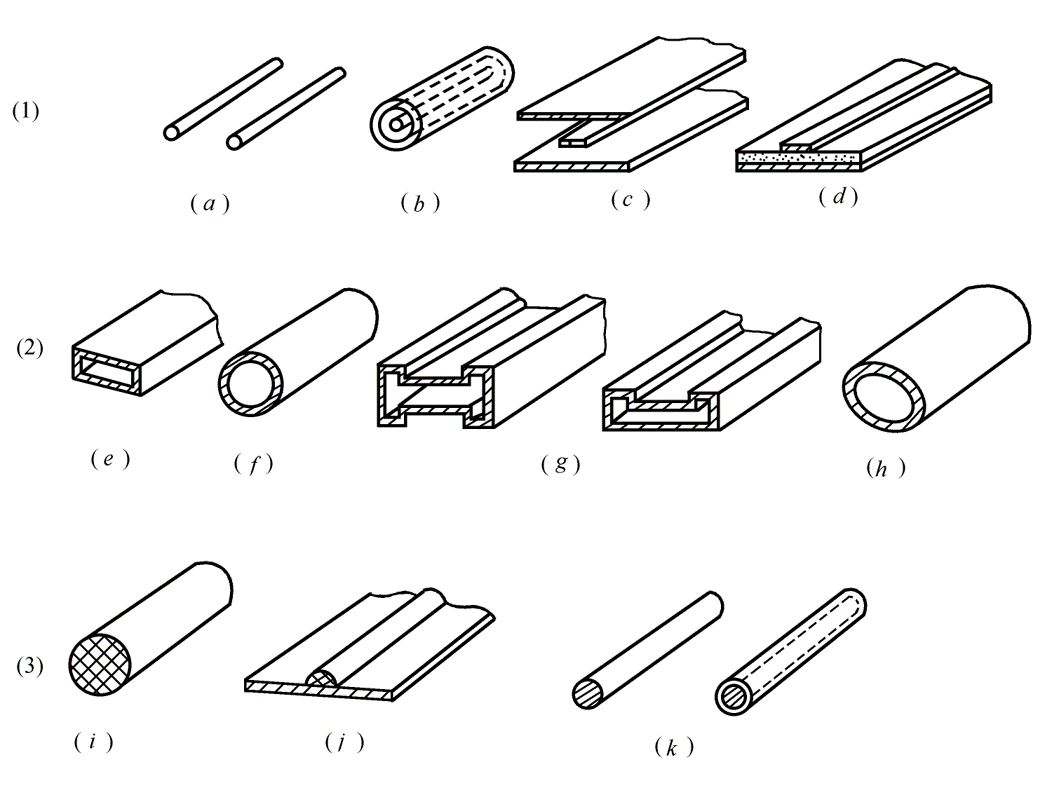
\includegraphics[width=9cm]{guidesystem.png}
  \saveenum
\end{frame}

\begin{frame}{传输线方程}
  \textbf{传输线}是以TEM导模的方式传送电磁波能量或信号的导行系统,其横向尺寸远小于其上工作波长。\\
  \textbf{传输线}有\textbf{长线}和\textbf{短线}之分。所谓长线是指传输线的几何长度与线上传输电磁波的波长比值(电长度)可相比拟,反之称为短线。\\
  \begin{align*}
    \text{长线}\Longrightarrow\text{分布参数电路}\\
    \text{短线}\Longrightarrow\text{集中参数电路}\\
    \text{分界线:}\widefbox{$l/\lambda\geq 0.05$}
  \end{align*}
  当频率提高到微波波段时,这些分布效应不可忽略,所以微波传输线是一种\textbf{分布参数电路}。这导致传输线上的电压和电流是随时间和空间位置而变化的二元函数。
\end{frame}

\begin{frame}{传输线方程}
  根据传输线上的分布参数是否均匀分布,可将其分为均匀传输线和不均匀传输线。我们可以把均匀传输线分割成许多小的微元段$dz(dz<<\lambda)$,这样每个微元段可以看作集中参数电路,用一个$\Gamma$型网络来等效。于是整个传输线可等效成无穷多个$\Gamma$型网络的级联。\\
  \centering
  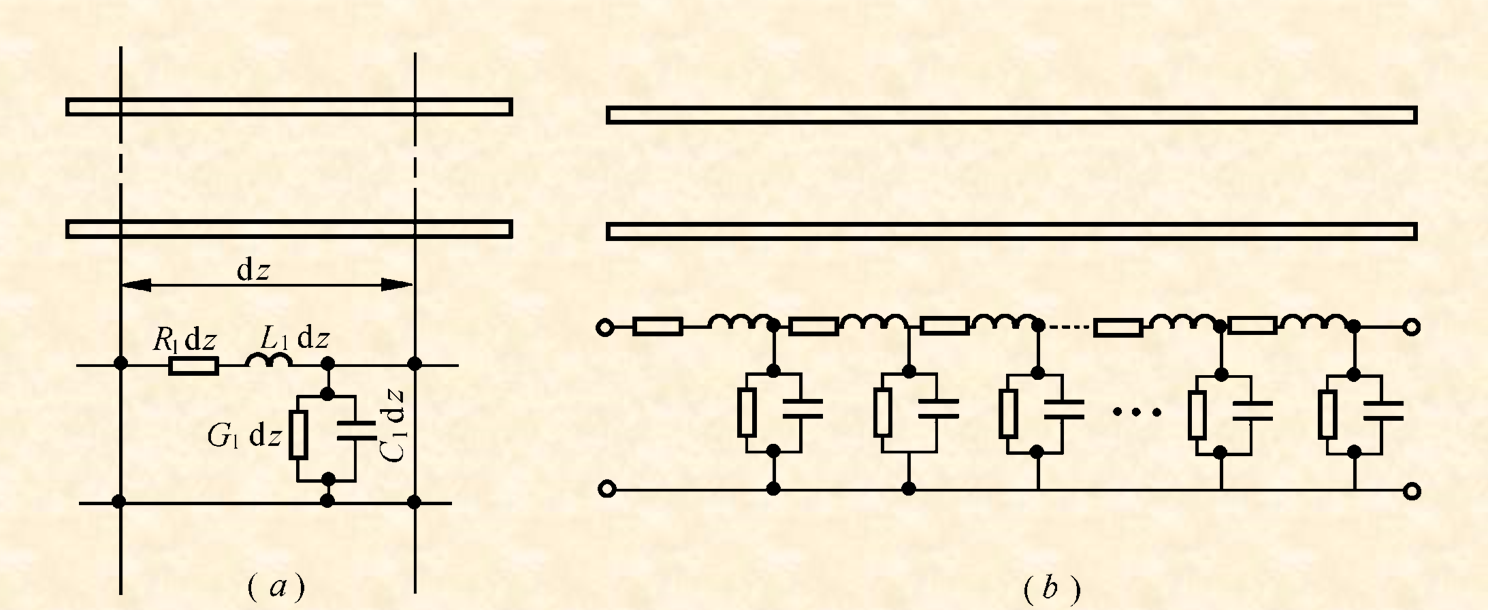
\includegraphics[width=9cm]{transmissionline1.png}
\end{frame}

\begin{frame}{传输线方程}
  双导线、同轴线和平行线传输线的分布参数\\
  \centering
  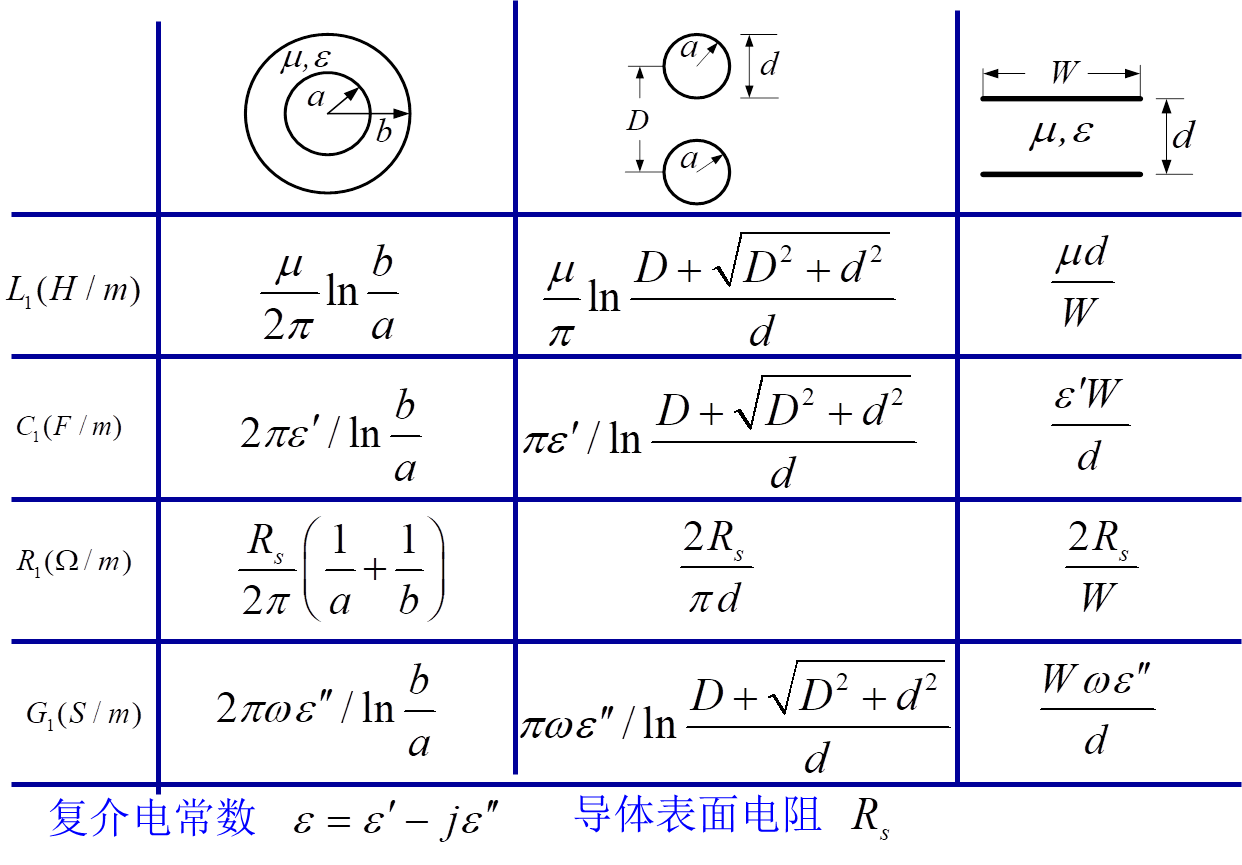
\includegraphics[width=9cm]{tmlineparas.png}
\end{frame}

\begin{frame}{传输线方程}
  \begin{enumerate}
    \resume
    \item 传输线方程\\
    
  \end{enumerate}
\end{frame}

\subsection{分布参数阻抗}
\begin{frame}{分布参数阻抗}

\end{frame}

\subsection{无耗线工作状态分析}
\begin{frame}{无耗线工作状态分析}

\end{frame}

\subsection{有耗线的特性与计算}
\begin{frame}{有耗线的特性与计算}

\end{frame}

\subsection{Smith Chart(阻抗圆图及其应用)}
\begin{frame}{Smith Chart(阻抗圆图及其应用)}

\end{frame}

\subsection{传输线的阻抗匹配}
\begin{frame}{传输线的阻抗匹配}

\end{frame}
